\documentclass[1p]{elsarticle_modified}
%\bibliographystyle{elsarticle-num}

%\usepackage[colorlinks]{hyperref}
%\usepackage{abbrmath_seonhwa} %\Abb, \Ascr, \Acal ,\Abf, \Afrak
\usepackage{amsfonts}
\usepackage{amssymb}
\usepackage{amsmath}
\usepackage{amsthm}
\usepackage{scalefnt}
\usepackage{amsbsy}
\usepackage{kotex}
\usepackage{caption}
\usepackage{subfig}
\usepackage{color}
\usepackage{graphicx}
\usepackage{xcolor} %% white, black, red, green, blue, cyan, magenta, yellow
\usepackage{float}
\usepackage{setspace}
\usepackage{hyperref}

\usepackage{tikz}
\usetikzlibrary{arrows}

\usepackage{multirow}
\usepackage{array} % fixed length table
\usepackage{hhline}

%%%%%%%%%%%%%%%%%%%%%
\makeatletter
\renewcommand*\env@matrix[1][\arraystretch]{%
	\edef\arraystretch{#1}%
	\hskip -\arraycolsep
	\let\@ifnextchar\new@ifnextchar
	\array{*\c@MaxMatrixCols c}}
\makeatother %https://tex.stackexchange.com/questions/14071/how-can-i-increase-the-line-spacing-in-a-matrix
%%%%%%%%%%%%%%%

\usepackage[normalem]{ulem}

\newcommand{\msout}[1]{\ifmmode\text{\sout{\ensuremath{#1}}}\else\sout{#1}\fi}
%SOURCE: \msout is \stkout macro in https://tex.stackexchange.com/questions/20609/strikeout-in-math-mode

\newcommand{\cancel}[1]{
	\ifmmode
	{\color{red}\msout{#1}}
	\else
	{\color{red}\sout{#1}}
	\fi
}

\newcommand{\add}[1]{
	{\color{blue}\uwave{#1}}
}

\newcommand{\replace}[2]{
	\ifmmode
	{\color{red}\msout{#1}}{\color{blue}\uwave{#2}}
	\else
	{\color{red}\sout{#1}}{\color{blue}\uwave{#2}}
	\fi
}

\newcommand{\Sol}{\mathcal{S}} %segment
\newcommand{\D}{D} %diagram
\newcommand{\A}{\mathcal{A}} %arc


%%%%%%%%%%%%%%%%%%%%%%%%%%%%%5 test

\def\sl{\operatorname{\textup{SL}}(2,\Cbb)}
\def\psl{\operatorname{\textup{PSL}}(2,\Cbb)}
\def\quan{\mkern 1mu \triangleright \mkern 1mu}

\theoremstyle{definition}
\newtheorem{thm}{Theorem}[section]
\newtheorem{prop}[thm]{Proposition}
\newtheorem{lem}[thm]{Lemma}
\newtheorem{ques}[thm]{Question}
\newtheorem{cor}[thm]{Corollary}
\newtheorem{defn}[thm]{Definition}
\newtheorem{exam}[thm]{Example}
\newtheorem{rmk}[thm]{Remark}
\newtheorem{alg}[thm]{Algorithm}

\newcommand{\I}{\sqrt{-1}}
\begin{document}

%\begin{frontmatter}
%
%\title{Boundary parabolic representations of knots up to 8 crossings}
%
%%% Group authors per affiliation:
%\author{Yunhi Cho} 
%\address{Department of Mathematics, University of Seoul, Seoul, Korea}
%\ead{yhcho@uos.ac.kr}
%
%
%\author{Seonhwa Kim} %\fnref{s_kim}}
%\address{Center for Geometry and Physics, Institute for Basic Science, Pohang, 37673, Korea}
%\ead{ryeona17@ibs.re.kr}
%
%\author{Hyuk Kim}
%\address{Department of Mathematical Sciences, Seoul National University, Seoul 08826, Korea}
%\ead{hyukkim@snu.ac.kr}
%
%\author{Seokbeom Yoon}
%\address{Department of Mathematical Sciences, Seoul National University, Seoul, 08826,  Korea}
%\ead{sbyoon15@snu.ac.kr}
%
%\begin{abstract}
%We find all boundary parabolic representation of knots up to 8 crossings.
%
%\end{abstract}
%\begin{keyword}
%    \MSC[2010] 57M25 
%\end{keyword}
%
%\end{frontmatter}

%\linenumbers
%\tableofcontents
%
\newcommand\colored[1]{\textcolor{white}{\rule[-0.35ex]{0.8em}{1.4ex}}\kern-0.8em\color{red} #1}%
%\newcommand\colored[1]{\textcolor{white}{ #1}\kern-2.17ex	\textcolor{white}{ #1}\kern-1.81ex	\textcolor{white}{ #1}\kern-2.15ex\color{red}#1	}

{\Large $\underline{12n_{0715}~(K12n_{0715})}$}

\setlength{\tabcolsep}{10pt}
\renewcommand{\arraystretch}{1.6}
\vspace{1cm}\begin{tabular}{m{100pt}>{\centering\arraybackslash}m{274pt}}
\multirow{5}{120pt}{
	\centering
	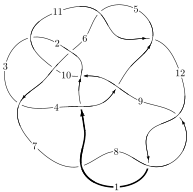
\includegraphics[width=112pt]{../../../GIT/diagram.site/Diagrams/png/2804_12n_0715.png}\\
\ \ \ A knot diagram\footnotemark}&
\allowdisplaybreaks
\textbf{Linearized knot diagam} \\
\cline{2-2}
 &
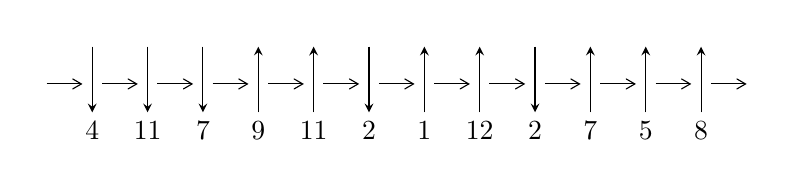
\begin{tikzpicture}[x=20pt, y=17pt]
	% nodes
	\node (C0) at (0, 0) {};
	\node (C1) at (1, 0) {};
	\node (C1U) at (1, +1) {};
	\node (C1D) at (1, -1) {4};

	\node (C2) at (2, 0) {};
	\node (C2U) at (2, +1) {};
	\node (C2D) at (2, -1) {11};

	\node (C3) at (3, 0) {};
	\node (C3U) at (3, +1) {};
	\node (C3D) at (3, -1) {7};

	\node (C4) at (4, 0) {};
	\node (C4U) at (4, +1) {};
	\node (C4D) at (4, -1) {9};

	\node (C5) at (5, 0) {};
	\node (C5U) at (5, +1) {};
	\node (C5D) at (5, -1) {11};

	\node (C6) at (6, 0) {};
	\node (C6U) at (6, +1) {};
	\node (C6D) at (6, -1) {2};

	\node (C7) at (7, 0) {};
	\node (C7U) at (7, +1) {};
	\node (C7D) at (7, -1) {1};

	\node (C8) at (8, 0) {};
	\node (C8U) at (8, +1) {};
	\node (C8D) at (8, -1) {12};

	\node (C9) at (9, 0) {};
	\node (C9U) at (9, +1) {};
	\node (C9D) at (9, -1) {2};

	\node (C10) at (10, 0) {};
	\node (C10U) at (10, +1) {};
	\node (C10D) at (10, -1) {7};

	\node (C11) at (11, 0) {};
	\node (C11U) at (11, +1) {};
	\node (C11D) at (11, -1) {5};

	\node (C12) at (12, 0) {};
	\node (C12U) at (12, +1) {};
	\node (C12D) at (12, -1) {8};
	\node (C13) at (13, 0) {};

	% arrows
	\draw[->,>={angle 60}]
	(C0) edge (C1) (C1) edge (C2) (C2) edge (C3) (C3) edge (C4) (C4) edge (C5) (C5) edge (C6) (C6) edge (C7) (C7) edge (C8) (C8) edge (C9) (C9) edge (C10) (C10) edge (C11) (C11) edge (C12) (C12) edge (C13) ;	\draw[->,>=stealth]
	(C1U) edge (C1D) (C2U) edge (C2D) (C3U) edge (C3D) (C4D) edge (C4U) (C5D) edge (C5U) (C6U) edge (C6D) (C7D) edge (C7U) (C8D) edge (C8U) (C9U) edge (C9D) (C10D) edge (C10U) (C11D) edge (C11U) (C12D) edge (C12U) ;
	\end{tikzpicture} \\
\hhline{~~} \\& 
\textbf{Solving Sequence} \\ \cline{2-2} 
 &
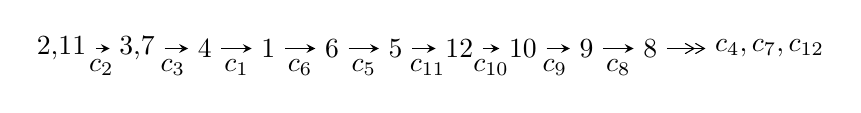
\begin{tikzpicture}[x=23pt, y=7pt]
	% node
	\node (A0) at (-1/8, 0) {2,11};
	\node (A1) at (17/16, 0) {3,7};
	\node (A2) at (17/8, 0) {4};
	\node (A3) at (25/8, 0) {1};
	\node (A4) at (33/8, 0) {6};
	\node (A5) at (41/8, 0) {5};
	\node (A6) at (49/8, 0) {12};
	\node (A7) at (57/8, 0) {10};
	\node (A8) at (65/8, 0) {9};
	\node (A9) at (73/8, 0) {8};
	\node (C1) at (1/2, -1) {$c_{2}$};
	\node (C2) at (13/8, -1) {$c_{3}$};
	\node (C3) at (21/8, -1) {$c_{1}$};
	\node (C4) at (29/8, -1) {$c_{6}$};
	\node (C5) at (37/8, -1) {$c_{5}$};
	\node (C6) at (45/8, -1) {$c_{11}$};
	\node (C7) at (53/8, -1) {$c_{10}$};
	\node (C8) at (61/8, -1) {$c_{9}$};
	\node (C9) at (69/8, -1) {$c_{8}$};
	\node (A10) at (11, 0) {$c_{4},c_{7},c_{12}$};

	% edge
	\draw[->,>=stealth]	
	(A0) edge (A1) (A1) edge (A2) (A2) edge (A3) (A3) edge (A4) (A4) edge (A5) (A5) edge (A6) (A6) edge (A7) (A7) edge (A8) (A8) edge (A9) ;
	\draw[->>,>={angle 60}]	
	(A9) edge (A10);
\end{tikzpicture} \\ 

\end{tabular} \\

\footnotetext{
The image of knot diagram is generated by the software ``\textbf{Draw programme}" developed by Andrew Bartholomew(\url{http://www.layer8.co.uk/maths/draw/index.htm\#Running-draw}), where we modified some parts for our purpose(\url{https://github.com/CATsTAILs/LinksPainter}).
}\phantom \\ \newline 
\centering \textbf{Ideals for irreducible components\footnotemark of $X_{\text{par}}$} 
 
\begin{align*}
I^u_{1}&=\langle 
4.60880\times10^{217} u^{59}+2.22932\times10^{217} u^{58}+\cdots+2.72986\times10^{221} b-9.04649\times10^{220},\\
\phantom{I^u_{1}}&\phantom{= \langle  }2.36217\times10^{222} u^{59}+8.17530\times10^{221} u^{58}+\cdots+8.32334\times10^{224} a+1.63524\times10^{225},\\
\phantom{I^u_{1}}&\phantom{= \langle  }u^{60}+31 u^{58}+\cdots-6806 u+3049\rangle \\
I^u_{2}&=\langle 
30594119 u^{15}-54613383 u^{14}+\cdots+339075961 b+341724092,\\
\phantom{I^u_{2}}&\phantom{= \langle  }-312874829 u^{15}+341866737 u^{14}+\cdots+339075961 a-448000694,\\
\phantom{I^u_{2}}&\phantom{= \langle  }u^{16}- u^{15}+5 u^{14}-3 u^{13}+10 u^{12}-7 u^{11}+u^{10}-3 u^9+10 u^8- u^7- u^6-3 u^5+11 u^4+3 u^3-4 u^2+1\rangle \\
\\
\end{align*}
\raggedright * 2 irreducible components of $\dim_{\mathbb{C}}=0$, with total 76 representations.\\
\footnotetext{All coefficients of polynomials are rational numbers. But the coefficients are sometimes approximated in decimal forms when there is not enough margin.}
\newpage
\renewcommand{\arraystretch}{1}
\centering \section*{I. $I^u_{1}= \langle 4.61\times10^{217} u^{59}+2.23\times10^{217} u^{58}+\cdots+2.73\times10^{221} b-9.05\times10^{220},\;2.36\times10^{222} u^{59}+8.18\times10^{221} u^{58}+\cdots+8.32\times10^{224} a+1.64\times10^{225},\;u^{60}+31 u^{58}+\cdots-6806 u+3049 \rangle$}
\flushleft \textbf{(i) Arc colorings}\\
\begin{tabular}{m{7pt} m{180pt} m{7pt} m{180pt} }
\flushright $a_{2}=$&$\begin{pmatrix}1\\0\end{pmatrix}$ \\
\flushright $a_{11}=$&$\begin{pmatrix}0\\u\end{pmatrix}$ \\
\flushright $a_{3}=$&$\begin{pmatrix}1\\u^2\end{pmatrix}$ \\
\flushright $a_{7}=$&$\begin{pmatrix}-0.00283801 u^{59}-0.000982214 u^{58}+\cdots-46.8813 u-1.96465\\-0.000168829 u^{59}-0.0000816642 u^{58}+\cdots-3.57585 u+0.331390\end{pmatrix}$ \\
\flushright $a_{4}=$&$\begin{pmatrix}-0.000945087 u^{59}+0.000227941 u^{58}+\cdots-22.2070 u+11.7845\\-0.000433429 u^{59}-0.000247835 u^{58}+\cdots-8.68770 u-0.364595\end{pmatrix}$ \\
\flushright $a_{1}=$&$\begin{pmatrix}0.000218505 u^{59}+0.000327052 u^{58}+\cdots+4.01660 u+3.62050\\0.000530540 u^{59}-0.0000863422 u^{58}+\cdots+10.7434 u-5.55537\end{pmatrix}$ \\
\flushright $a_{6}=$&$\begin{pmatrix}-0.00300684 u^{59}-0.00106388 u^{58}+\cdots-50.4571 u-1.63326\\-0.000168829 u^{59}-0.0000816642 u^{58}+\cdots-3.57585 u+0.331390\end{pmatrix}$ \\
\flushright $a_{5}=$&$\begin{pmatrix}-0.00300684 u^{59}-0.00106388 u^{58}+\cdots-50.4571 u-1.63326\\-0.0000163342 u^{59}+0.000121229 u^{58}+\cdots-1.64875 u+3.57516\end{pmatrix}$ \\
\flushright $a_{12}=$&$\begin{pmatrix}0.000720153 u^{59}-0.000752234 u^{58}+\cdots+22.6935 u-14.1062\\-0.000822043 u^{59}+0.000203348 u^{58}+\cdots-15.0493 u+9.22217\end{pmatrix}$ \\
\flushright $a_{10}=$&$\begin{pmatrix}-0.00155459 u^{59}+0.00108020 u^{58}+\cdots-39.1669 u+27.2099\\0.000345116 u^{59}-0.000186298 u^{58}+\cdots+8.73955 u-6.17511\end{pmatrix}$ \\
\flushright $a_{9}=$&$\begin{pmatrix}-0.00120947 u^{59}+0.000893904 u^{58}+\cdots-30.4274 u+21.0348\\0.000345116 u^{59}-0.000186298 u^{58}+\cdots+8.73955 u-6.17511\end{pmatrix}$ \\
\flushright $a_{8}=$&$\begin{pmatrix}-0.00175525 u^{59}-0.000468763 u^{58}+\cdots-34.3728 u+3.63194\\0.000128794 u^{59}-0.000138534 u^{58}+\cdots+3.06900 u-1.69755\end{pmatrix}$\\&\end{tabular}
\flushleft \textbf{(ii) Obstruction class $= -1$}\\~\\
\flushleft \textbf{(iii) Cusp Shapes $= 0.00272374 u^{59}+0.00105874 u^{58}+\cdots+53.4296 u-4.72817$}\\~\\
\newpage\renewcommand{\arraystretch}{1}
\flushleft \textbf{(iv) u-Polynomials at the component}\newline \\
\begin{tabular}{m{50pt}|m{274pt}}
Crossings & \hspace{64pt}u-Polynomials at each crossing \\
\hline $$\begin{aligned}c_{1}\end{aligned}$$&$\begin{aligned}
&u^{60}-8 u^{59}+\cdots-27 u+1
\end{aligned}$\\
\hline $$\begin{aligned}c_{2}\end{aligned}$$&$\begin{aligned}
&u^{60}+31 u^{58}+\cdots+6806 u+3049
\end{aligned}$\\
\hline $$\begin{aligned}c_{3}\end{aligned}$$&$\begin{aligned}
&u^{60}-4 u^{58}+\cdots+905 u+79
\end{aligned}$\\
\hline $$\begin{aligned}c_{4}\end{aligned}$$&$\begin{aligned}
&u^{60}+3 u^{59}+\cdots+6612 u+977
\end{aligned}$\\
\hline $$\begin{aligned}c_{5},c_{11}\end{aligned}$$&$\begin{aligned}
&u^{60}+19 u^{58}+\cdots+1808 u+136
\end{aligned}$\\
\hline $$\begin{aligned}c_{6}\end{aligned}$$&$\begin{aligned}
&u^{60}+3 u^{59}+\cdots+5062 u+484
\end{aligned}$\\
\hline $$\begin{aligned}c_{7},c_{8},c_{12}\end{aligned}$$&$\begin{aligned}
&u^{60}-2 u^{59}+\cdots+12 u+1
\end{aligned}$\\
\hline $$\begin{aligned}c_{9}\end{aligned}$$&$\begin{aligned}
&u^{60}-4 u^{59}+\cdots+232 u+8
\end{aligned}$\\
\hline $$\begin{aligned}c_{10}\end{aligned}$$&$\begin{aligned}
&u^{60}+3 u^{59}+\cdots+1069 u+541
\end{aligned}$\\
\hline
\end{tabular}\\~\\
\newpage\renewcommand{\arraystretch}{1}
\flushleft \textbf{(v) Riley Polynomials at the component}\newline \\
\begin{tabular}{m{50pt}|m{274pt}}
Crossings & \hspace{64pt}Riley Polynomials at each crossing \\
\hline $$\begin{aligned}c_{1}\end{aligned}$$&$\begin{aligned}
&y^{60}+2 y^{59}+\cdots-233 y+1
\end{aligned}$\\
\hline $$\begin{aligned}c_{2}\end{aligned}$$&$\begin{aligned}
&y^{60}+62 y^{59}+\cdots+271621986 y+9296401
\end{aligned}$\\
\hline $$\begin{aligned}c_{3}\end{aligned}$$&$\begin{aligned}
&y^{60}-8 y^{59}+\cdots-193345 y+6241
\end{aligned}$\\
\hline $$\begin{aligned}c_{4}\end{aligned}$$&$\begin{aligned}
&y^{60}+21 y^{59}+\cdots+18369806 y+954529
\end{aligned}$\\
\hline $$\begin{aligned}c_{5},c_{11}\end{aligned}$$&$\begin{aligned}
&y^{60}+38 y^{59}+\cdots-152832 y+18496
\end{aligned}$\\
\hline $$\begin{aligned}c_{6}\end{aligned}$$&$\begin{aligned}
&y^{60}+63 y^{59}+\cdots+4369636 y+234256
\end{aligned}$\\
\hline $$\begin{aligned}c_{7},c_{8},c_{12}\end{aligned}$$&$\begin{aligned}
&y^{60}+64 y^{59}+\cdots-6 y+1
\end{aligned}$\\
\hline $$\begin{aligned}c_{9}\end{aligned}$$&$\begin{aligned}
&y^{60}+14 y^{59}+\cdots+2240 y+64
\end{aligned}$\\
\hline $$\begin{aligned}c_{10}\end{aligned}$$&$\begin{aligned}
&y^{60}-75 y^{59}+\cdots-4777199 y+292681
\end{aligned}$\\
\hline
\end{tabular}\\~\\
\newpage\flushleft \textbf{(vi) Complex Volumes and Cusp Shapes}
$$\begin{array}{c|c|c}  
\text{Solutions to }I^u_{1}& \I (\text{vol} + \sqrt{-1}CS) & \text{Cusp shape}\\
 \hline 
\begin{aligned}
u &= \phantom{-}0.643501 + 0.773438 I \\
a &= \phantom{-}0.477987 - 0.525534 I \\
b &= -0.480857 + 0.417860 I\end{aligned}
 & -1.32280 - 2.56367 I & \phantom{-}5.00187 + 5.20719 I \\ \hline\begin{aligned}
u &= \phantom{-}0.643501 - 0.773438 I \\
a &= \phantom{-}0.477987 + 0.525534 I \\
b &= -0.480857 - 0.417860 I\end{aligned}
 & -1.32280 + 2.56367 I & \phantom{-}5.00187 - 5.20719 I \\ \hline\begin{aligned}
u &= \phantom{-}0.926449 + 0.415748 I \\
a &= \phantom{-}0.352525 + 0.205719 I \\
b &= \phantom{-}0.272409 + 0.505392 I\end{aligned}
 & -1.76277 - 1.27508 I & \phantom{-}3.66951 + 0. I\phantom{ +0.000000I} \\ \hline\begin{aligned}
u &= \phantom{-}0.926449 - 0.415748 I \\
a &= \phantom{-}0.352525 - 0.205719 I \\
b &= \phantom{-}0.272409 - 0.505392 I\end{aligned}
 & -1.76277 + 1.27508 I & \phantom{-}3.66951 + 0. I\phantom{ +0.000000I} \\ \hline\begin{aligned}
u &= \phantom{-}0.053170 + 0.925086 I \\
a &= \phantom{-}0.623976 - 0.343376 I \\
b &= -1.53558 + 0.06817 I\end{aligned}
 & -1.87416 - 3.34982 I & -1.36055 + 8.15563 I \\ \hline\begin{aligned}
u &= \phantom{-}0.053170 - 0.925086 I \\
a &= \phantom{-}0.623976 + 0.343376 I \\
b &= -1.53558 - 0.06817 I\end{aligned}
 & -1.87416 + 3.34982 I & -1.36055 - 8.15563 I \\ \hline\begin{aligned}
u &= -0.500509 + 0.765670 I \\
a &= -1.83740 - 0.54894 I \\
b &= \phantom{-}0.75841 + 1.43263 I\end{aligned}
 & -4.99862 + 3.16468 I & -14.6216 - 8.5416 I \\ \hline\begin{aligned}
u &= -0.500509 - 0.765670 I \\
a &= -1.83740 + 0.54894 I \\
b &= \phantom{-}0.75841 - 1.43263 I\end{aligned}
 & -4.99862 - 3.16468 I & -14.6216 + 8.5416 I \\ \hline\begin{aligned}
u &= \phantom{-}0.034645 + 0.884579 I \\
a &= \phantom{-}0.286455 + 0.321976 I \\
b &= -1.59579 + 0.20592 I\end{aligned}
 & -9.60436 + 7.44720 I & -1.12455 - 5.22316 I \\ \hline\begin{aligned}
u &= \phantom{-}0.034645 - 0.884579 I \\
a &= \phantom{-}0.286455 - 0.321976 I \\
b &= -1.59579 - 0.20592 I\end{aligned}
 & -9.60436 - 7.44720 I & -1.12455 + 5.22316 I\\
 \hline 
 \end{array}$$\newpage$$\begin{array}{c|c|c}  
\text{Solutions to }I^u_{1}& \I (\text{vol} + \sqrt{-1}CS) & \text{Cusp shape}\\
 \hline 
\begin{aligned}
u &= -0.544528 + 1.008840 I \\
a &= \phantom{-}0.813613 - 0.130165 I \\
b &= \phantom{-}0.488628 - 0.533810 I\end{aligned}
 & -6.88275 + 2.17208 I & \phantom{-0.000000 } 0 \\ \hline\begin{aligned}
u &= -0.544528 - 1.008840 I \\
a &= \phantom{-}0.813613 + 0.130165 I \\
b &= \phantom{-}0.488628 + 0.533810 I\end{aligned}
 & -6.88275 - 2.17208 I & \phantom{-0.000000 } 0 \\ \hline\begin{aligned}
u &= -0.318234 + 1.129480 I \\
a &= -0.32972 - 1.56989 I \\
b &= -0.46348 + 1.86984 I\end{aligned}
 & -3.89674 + 0.34222 I & \phantom{-0.000000 } 0 \\ \hline\begin{aligned}
u &= -0.318234 - 1.129480 I \\
a &= -0.32972 + 1.56989 I \\
b &= -0.46348 - 1.86984 I\end{aligned}
 & -3.89674 - 0.34222 I & \phantom{-0.000000 } 0 \\ \hline\begin{aligned}
u &= -0.378871 + 0.636122 I \\
a &= -2.18887 + 0.97531 I \\
b &= \phantom{-}0.262076 - 0.282529 I\end{aligned}
 & -10.56020 - 6.42506 I & \phantom{-}0.29601 + 1.69572 I \\ \hline\begin{aligned}
u &= -0.378871 - 0.636122 I \\
a &= -2.18887 - 0.97531 I \\
b &= \phantom{-}0.262076 + 0.282529 I\end{aligned}
 & -10.56020 + 6.42506 I & \phantom{-}0.29601 - 1.69572 I \\ \hline\begin{aligned}
u &= \phantom{-}0.596985 + 0.415802 I \\
a &= \phantom{-}0.630468 + 0.640731 I \\
b &= \phantom{-}0.421600 + 0.581478 I\end{aligned}
 & -1.70945 - 1.35880 I & \phantom{-}2.24467 + 5.29357 I \\ \hline\begin{aligned}
u &= \phantom{-}0.596985 - 0.415802 I \\
a &= \phantom{-}0.630468 - 0.640731 I \\
b &= \phantom{-}0.421600 - 0.581478 I\end{aligned}
 & -1.70945 + 1.35880 I & \phantom{-}2.24467 - 5.29357 I \\ \hline\begin{aligned}
u &= -1.295930 + 0.133460 I \\
a &= -0.279441 + 0.102123 I \\
b &= \phantom{-}0.068794 - 0.818384 I\end{aligned}
 & -1.99077 + 4.39001 I & \phantom{-0.000000 } 0 \\ \hline\begin{aligned}
u &= -1.295930 - 0.133460 I \\
a &= -0.279441 - 0.102123 I \\
b &= \phantom{-}0.068794 + 0.818384 I\end{aligned}
 & -1.99077 - 4.39001 I & \phantom{-0.000000 } 0\\
 \hline 
 \end{array}$$\newpage$$\begin{array}{c|c|c}  
\text{Solutions to }I^u_{1}& \I (\text{vol} + \sqrt{-1}CS) & \text{Cusp shape}\\
 \hline 
\begin{aligned}
u &= -0.540732 + 0.427519 I \\
a &= \phantom{-}0.760586 + 0.277873 I \\
b &= \phantom{-}1.34981 - 0.58688 I\end{aligned}
 & -8.08596 + 1.79714 I & \phantom{-}2.34826 - 0.92148 I \\ \hline\begin{aligned}
u &= -0.540732 - 0.427519 I \\
a &= \phantom{-}0.760586 - 0.277873 I \\
b &= \phantom{-}1.34981 + 0.58688 I\end{aligned}
 & -8.08596 - 1.79714 I & \phantom{-}2.34826 + 0.92148 I \\ \hline\begin{aligned}
u &= \phantom{-}0.345641 + 0.471474 I \\
a &= \phantom{-}1.388840 - 0.024076 I \\
b &= \phantom{-}0.015962 - 0.605849 I\end{aligned}
 & -4.31256 + 2.44729 I & \phantom{-}0.28400 - 3.32996 I \\ \hline\begin{aligned}
u &= \phantom{-}0.345641 - 0.471474 I \\
a &= \phantom{-}1.388840 + 0.024076 I \\
b &= \phantom{-}0.015962 + 0.605849 I\end{aligned}
 & -4.31256 - 2.44729 I & \phantom{-}0.28400 + 3.32996 I \\ \hline\begin{aligned}
u &= -1.29147 + 0.58402 I \\
a &= \phantom{-}0.565494 - 0.060409 I \\
b &= \phantom{-}0.438216 - 0.286617 I\end{aligned}
 & -7.55798 + 1.00360 I & \phantom{-0.000000 } 0 \\ \hline\begin{aligned}
u &= -1.29147 - 0.58402 I \\
a &= \phantom{-}0.565494 + 0.060409 I \\
b &= \phantom{-}0.438216 + 0.286617 I\end{aligned}
 & -7.55798 - 1.00360 I & \phantom{-0.000000 } 0 \\ \hline\begin{aligned}
u &= \phantom{-}0.05414 + 1.42407 I \\
a &= -0.319172 + 1.234000 I \\
b &= -0.01533 - 1.75620 I\end{aligned}
 & \phantom{-}6.16440 + 0.67247 I & \phantom{-0.000000 } 0 \\ \hline\begin{aligned}
u &= \phantom{-}0.05414 - 1.42407 I \\
a &= -0.319172 - 1.234000 I \\
b &= -0.01533 + 1.75620 I\end{aligned}
 & \phantom{-}6.16440 - 0.67247 I & \phantom{-0.000000 } 0 \\ \hline\begin{aligned}
u &= -0.298967 + 0.388601 I \\
a &= \phantom{-}1.068600 + 0.374239 I \\
b &= -0.238474 + 0.258177 I\end{aligned}
 & \phantom{-}1.029620 - 0.495284 I & \phantom{-}8.01687 + 2.31808 I \\ \hline\begin{aligned}
u &= -0.298967 - 0.388601 I \\
a &= \phantom{-}1.068600 - 0.374239 I \\
b &= -0.238474 - 0.258177 I\end{aligned}
 & \phantom{-}1.029620 + 0.495284 I & \phantom{-}8.01687 - 2.31808 I\\
 \hline 
 \end{array}$$\newpage$$\begin{array}{c|c|c}  
\text{Solutions to }I^u_{1}& \I (\text{vol} + \sqrt{-1}CS) & \text{Cusp shape}\\
 \hline 
\begin{aligned}
u &= \phantom{-}0.32296 + 1.49533 I \\
a &= -0.014077 + 1.294100 I \\
b &= -0.62950 - 1.74634 I\end{aligned}
 & \phantom{-}4.16311 - 5.16210 I & \phantom{-0.000000 } 0 \\ \hline\begin{aligned}
u &= \phantom{-}0.32296 - 1.49533 I \\
a &= -0.014077 - 1.294100 I \\
b &= -0.62950 + 1.74634 I\end{aligned}
 & \phantom{-}4.16311 + 5.16210 I & \phantom{-0.000000 } 0 \\ \hline\begin{aligned}
u &= \phantom{-}1.53276 + 0.02218 I \\
a &= -0.430876 + 0.228519 I \\
b &= \phantom{-}0.008534 - 0.918471 I\end{aligned}
 & -8.47818 + 7.22559 I & \phantom{-0.000000 } 0 \\ \hline\begin{aligned}
u &= \phantom{-}1.53276 - 0.02218 I \\
a &= -0.430876 - 0.228519 I \\
b &= \phantom{-}0.008534 + 0.918471 I\end{aligned}
 & -8.47818 - 7.22559 I & \phantom{-0.000000 } 0 \\ \hline\begin{aligned}
u &= \phantom{-}0.160181 + 0.387104 I \\
a &= -3.57956 - 1.20981 I \\
b &= \phantom{-}0.505995 + 0.337305 I\end{aligned}
 & -3.56642 + 2.79917 I & \phantom{-}3.42811 - 0.46170 I \\ \hline\begin{aligned}
u &= \phantom{-}0.160181 - 0.387104 I \\
a &= -3.57956 + 1.20981 I \\
b &= \phantom{-}0.505995 - 0.337305 I\end{aligned}
 & -3.56642 - 2.79917 I & \phantom{-}3.42811 + 0.46170 I \\ \hline\begin{aligned}
u &= \phantom{-}0.206989 + 0.338042 I \\
a &= \phantom{-}1.055210 - 0.169889 I \\
b &= \phantom{-}0.929185 + 0.315681 I\end{aligned}
 & -1.68988 - 0.84367 I & -1.15133 - 2.48572 I \\ \hline\begin{aligned}
u &= \phantom{-}0.206989 - 0.338042 I \\
a &= \phantom{-}1.055210 + 0.169889 I \\
b &= \phantom{-}0.929185 - 0.315681 I\end{aligned}
 & -1.68988 + 0.84367 I & -1.15133 + 2.48572 I \\ \hline\begin{aligned}
u &= -0.53294 + 1.53814 I \\
a &= \phantom{-}0.207126 + 0.755558 I \\
b &= \phantom{-}0.57668 - 1.68015 I\end{aligned}
 & -3.90465 + 5.68518 I & \phantom{-0.000000 } 0 \\ \hline\begin{aligned}
u &= -0.53294 - 1.53814 I \\
a &= \phantom{-}0.207126 - 0.755558 I \\
b &= \phantom{-}0.57668 + 1.68015 I\end{aligned}
 & -3.90465 - 5.68518 I & \phantom{-0.000000 } 0\\
 \hline 
 \end{array}$$\newpage$$\begin{array}{c|c|c}  
\text{Solutions to }I^u_{1}& \I (\text{vol} + \sqrt{-1}CS) & \text{Cusp shape}\\
 \hline 
\begin{aligned}
u &= -0.34251 + 1.60989 I \\
a &= \phantom{-}0.257663 - 1.104060 I \\
b &= \phantom{-}0.313142 + 1.134510 I\end{aligned}
 & -0.04200 + 2.46645 I & \phantom{-0.000000 } 0 \\ \hline\begin{aligned}
u &= -0.34251 - 1.60989 I \\
a &= \phantom{-}0.257663 + 1.104060 I \\
b &= \phantom{-}0.313142 - 1.134510 I\end{aligned}
 & -0.04200 - 2.46645 I & \phantom{-0.000000 } 0 \\ \hline\begin{aligned}
u &= \phantom{-}0.37318 + 1.63255 I \\
a &= \phantom{-}0.196758 - 0.879828 I \\
b &= \phantom{-}0.39480 + 1.54627 I\end{aligned}
 & \phantom{-}2.93179 - 4.03578 I & \phantom{-0.000000 } 0 \\ \hline\begin{aligned}
u &= \phantom{-}0.37318 - 1.63255 I \\
a &= \phantom{-}0.196758 + 0.879828 I \\
b &= \phantom{-}0.39480 - 1.54627 I\end{aligned}
 & \phantom{-}2.93179 + 4.03578 I & \phantom{-0.000000 } 0 \\ \hline\begin{aligned}
u &= \phantom{-}0.07899 + 1.69652 I \\
a &= -0.205758 - 1.016470 I \\
b &= \phantom{-}0.04852 + 1.75392 I\end{aligned}
 & \phantom{-}7.60928 - 4.45168 I & \phantom{-0.000000 } 0 \\ \hline\begin{aligned}
u &= \phantom{-}0.07899 - 1.69652 I \\
a &= -0.205758 + 1.016470 I \\
b &= \phantom{-}0.04852 - 1.75392 I\end{aligned}
 & \phantom{-}7.60928 + 4.45168 I & \phantom{-0.000000 } 0 \\ \hline\begin{aligned}
u &= -0.48846 + 1.64668 I \\
a &= -0.076786 - 1.162360 I \\
b &= -0.55112 + 1.73815 I\end{aligned}
 & \phantom{-}4.09640 + 10.99650 I & \phantom{-0.000000 } 0 \\ \hline\begin{aligned}
u &= -0.48846 - 1.64668 I \\
a &= -0.076786 + 1.162360 I \\
b &= -0.55112 - 1.73815 I\end{aligned}
 & \phantom{-}4.09640 - 10.99650 I & \phantom{-0.000000 } 0 \\ \hline\begin{aligned}
u &= \phantom{-}0.95133 + 1.45075 I \\
a &= \phantom{-}0.334549 - 1.088470 I \\
b &= \phantom{-}0.08628 + 1.49845 I\end{aligned}
 & -0.33304 - 4.22189 I & \phantom{-0.000000 } 0 \\ \hline\begin{aligned}
u &= \phantom{-}0.95133 - 1.45075 I \\
a &= \phantom{-}0.334549 + 1.088470 I \\
b &= \phantom{-}0.08628 - 1.49845 I\end{aligned}
 & -0.33304 + 4.22189 I & \phantom{-0.000000 } 0\\
 \hline 
 \end{array}$$\newpage$$\begin{array}{c|c|c}  
\text{Solutions to }I^u_{1}& \I (\text{vol} + \sqrt{-1}CS) & \text{Cusp shape}\\
 \hline 
\begin{aligned}
u &= -0.67460 + 1.61393 I \\
a &= \phantom{-}0.214492 + 1.072810 I \\
b &= \phantom{-}0.09563 - 1.53472 I\end{aligned}
 & \phantom{-}5.14342 + 3.33363 I & \phantom{-0.000000 } 0 \\ \hline\begin{aligned}
u &= -0.67460 - 1.61393 I \\
a &= \phantom{-}0.214492 - 1.072810 I \\
b &= \phantom{-}0.09563 + 1.53472 I\end{aligned}
 & \phantom{-}5.14342 - 3.33363 I & \phantom{-0.000000 } 0 \\ \hline\begin{aligned}
u &= -0.05843 + 1.75203 I \\
a &= \phantom{-}0.238224 + 0.996234 I \\
b &= \phantom{-}0.301077 - 1.305630 I\end{aligned}
 & \phantom{-}4.54407 + 0.89244 I & \phantom{-0.000000 } 0 \\ \hline\begin{aligned}
u &= -0.05843 - 1.75203 I \\
a &= \phantom{-}0.238224 - 0.996234 I \\
b &= \phantom{-}0.301077 + 1.305630 I\end{aligned}
 & \phantom{-}4.54407 - 0.89244 I & \phantom{-0.000000 } 0 \\ \hline\begin{aligned}
u &= \phantom{-}0.64109 + 1.69574 I \\
a &= -0.124519 + 1.104800 I \\
b &= -0.52332 - 1.76203 I\end{aligned}
 & -2.9040 - 15.1991 I & \phantom{-0.000000 } 0 \\ \hline\begin{aligned}
u &= \phantom{-}0.64109 - 1.69574 I \\
a &= -0.124519 - 1.104800 I \\
b &= -0.52332 + 1.76203 I\end{aligned}
 & -2.9040 + 15.1991 I & \phantom{-0.000000 } 0 \\ \hline\begin{aligned}
u &= -0.18386 + 1.88121 I \\
a &= -0.161769 + 0.888934 I \\
b &= \phantom{-}0.08443 - 1.80565 I\end{aligned}
 & \phantom{-}1.96683 + 7.20981 I & \phantom{-0.000000 } 0 \\ \hline\begin{aligned}
u &= -0.18386 - 1.88121 I \\
a &= -0.161769 - 0.888934 I \\
b &= \phantom{-}0.08443 + 1.80565 I\end{aligned}
 & \phantom{-}1.96683 - 7.20981 I & \phantom{-0.000000 } 0 \\ \hline\begin{aligned}
u &= \phantom{-}0.52803 + 1.98863 I \\
a &= \phantom{-}0.197232 - 0.978791 I \\
b &= \phantom{-}0.11327 + 1.46699 I\end{aligned}
 & \phantom{-}1.77020 - 3.01560 I & \phantom{-0.000000 } 0 \\ \hline\begin{aligned}
u &= \phantom{-}0.52803 - 1.98863 I \\
a &= \phantom{-}0.197232 + 0.978791 I \\
b &= \phantom{-}0.11327 - 1.46699 I\end{aligned}
 & \phantom{-}1.77020 + 3.01560 I & \phantom{-0.000000 } 0\\
 \hline 
 \end{array}$$\newpage\newpage\renewcommand{\arraystretch}{1}
\centering \section*{II. $I^u_{2}= \langle 3.06\times10^{7} u^{15}-5.46\times10^{7} u^{14}+\cdots+3.39\times10^{8} b+3.42\times10^{8},\;-3.13\times10^{8} u^{15}+3.42\times10^{8} u^{14}+\cdots+3.39\times10^{8} a-4.48\times10^{8},\;u^{16}- u^{15}+\cdots-4 u^2+1 \rangle$}
\flushleft \textbf{(i) Arc colorings}\\
\begin{tabular}{m{7pt} m{180pt} m{7pt} m{180pt} }
\flushright $a_{2}=$&$\begin{pmatrix}1\\0\end{pmatrix}$ \\
\flushright $a_{11}=$&$\begin{pmatrix}0\\u\end{pmatrix}$ \\
\flushright $a_{3}=$&$\begin{pmatrix}1\\u^2\end{pmatrix}$ \\
\flushright $a_{7}=$&$\begin{pmatrix}0.922728 u^{15}-1.00823 u^{14}+\cdots+1.66385 u+1.32124\\-0.0902279 u^{15}+0.161065 u^{14}+\cdots+0.181578 u-1.00781\end{pmatrix}$ \\
\flushright $a_{4}=$&$\begin{pmatrix}-0.832500 u^{15}+0.847165 u^{14}+\cdots-1.84543 u+1.68657\\0.402236 u^{15}-0.549776 u^{14}+\cdots-0.832500 u+1.01467\end{pmatrix}$ \\
\flushright $a_{1}=$&$\begin{pmatrix}-0.555116 u^{15}+0.977164 u^{14}+\cdots+4.61473 u-2.80921\\-0.661929 u^{15}+1.03099 u^{14}+\cdots+1.18736 u-0.951848\end{pmatrix}$ \\
\flushright $a_{6}=$&$\begin{pmatrix}0.832500 u^{15}-0.847165 u^{14}+\cdots+1.84543 u+0.313430\\-0.0902279 u^{15}+0.161065 u^{14}+\cdots+0.181578 u-1.00781\end{pmatrix}$ \\
\flushright $a_{5}=$&$\begin{pmatrix}0.832500 u^{15}-0.847165 u^{14}+\cdots+1.84543 u+0.313430\\0.312008 u^{15}-0.388710 u^{14}+\cdots-0.650922 u-0.993145\end{pmatrix}$ \\
\flushright $a_{12}=$&$\begin{pmatrix}1.94577 u^{15}-2.42341 u^{14}+\cdots-7.34438 u+0.702070\\0.0154462 u^{15}-0.545396 u^{14}+\cdots-1.25235 u+0.998126\end{pmatrix}$ \\
\flushright $a_{10}=$&$\begin{pmatrix}-1.92294 u^{15}+1.59142 u^{14}+\cdots+5.80143 u+0.319406\\-0.0848705 u^{15}+0.506614 u^{14}+\cdots+2.23637 u-0.500984\end{pmatrix}$ \\
\flushright $a_{9}=$&$\begin{pmatrix}-2.00781 u^{15}+2.09804 u^{14}+\cdots+8.03780 u-0.181578\\-0.0848705 u^{15}+0.506614 u^{14}+\cdots+2.23637 u-0.500984\end{pmatrix}$ \\
\flushright $a_{8}=$&$\begin{pmatrix}-1.32494 u^{15}+2.35544 u^{14}+\cdots+3.78101 u-0.969814\\0.286898 u^{15}-0.131334 u^{14}+\cdots-1.86529 u+0.366755\end{pmatrix}$\\&\end{tabular}
\flushleft \textbf{(ii) Obstruction class $= 1$}\\~\\
\flushleft \textbf{(iii) Cusp Shapes $= \frac{1384808610}{339075961} u^{15}-\frac{1263687753}{339075961} u^{14}+\cdots+\frac{226684056}{339075961} u-\frac{2103842549}{339075961}$}\\~\\
\newpage\renewcommand{\arraystretch}{1}
\flushleft \textbf{(iv) u-Polynomials at the component}\newline \\
\begin{tabular}{m{50pt}|m{274pt}}
Crossings & \hspace{64pt}u-Polynomials at each crossing \\
\hline $$\begin{aligned}c_{1}\end{aligned}$$&$\begin{aligned}
&u^{16}-7 u^{15}+\cdots-3 u+1
\end{aligned}$\\
\hline $$\begin{aligned}c_{2}\end{aligned}$$&$\begin{aligned}
&u^{16}- u^{15}+\cdots-4 u^2+1
\end{aligned}$\\
\hline $$\begin{aligned}c_{3}\end{aligned}$$&$\begin{aligned}
&u^{16}+5 u^{15}+\cdots+7 u+1
\end{aligned}$\\
\hline $$\begin{aligned}c_{4}\end{aligned}$$&$\begin{aligned}
&u^{16}+2 u^{14}+\cdots+4 u+1
\end{aligned}$\\
\hline $$\begin{aligned}c_{5}\end{aligned}$$&$\begin{aligned}
&u^{16}- u^{15}+\cdots+8 u+8
\end{aligned}$\\
\hline $$\begin{aligned}c_{6}\end{aligned}$$&$\begin{aligned}
&u^{16}+2 u^{15}+\cdots+2 u+4
\end{aligned}$\\
\hline $$\begin{aligned}c_{7},c_{8}\end{aligned}$$&$\begin{aligned}
&u^{16}- u^{15}+\cdots+2 u+1
\end{aligned}$\\
\hline $$\begin{aligned}c_{9}\end{aligned}$$&$\begin{aligned}
&u^{16}+3 u^{15}+\cdots-12 u^2+8
\end{aligned}$\\
\hline $$\begin{aligned}c_{10}\end{aligned}$$&$\begin{aligned}
&u^{16}+4 u^{15}+\cdots+7 u+1
\end{aligned}$\\
\hline $$\begin{aligned}c_{11}\end{aligned}$$&$\begin{aligned}
&u^{16}+u^{15}+\cdots-8 u+8
\end{aligned}$\\
\hline $$\begin{aligned}c_{12}\end{aligned}$$&$\begin{aligned}
&u^{16}+u^{15}+\cdots-2 u+1
\end{aligned}$\\
\hline
\end{tabular}\\~\\
\newpage\renewcommand{\arraystretch}{1}
\flushleft \textbf{(v) Riley Polynomials at the component}\newline \\
\begin{tabular}{m{50pt}|m{274pt}}
Crossings & \hspace{64pt}Riley Polynomials at each crossing \\
\hline $$\begin{aligned}c_{1}\end{aligned}$$&$\begin{aligned}
&y^{16}+y^{15}+\cdots+5 y+1
\end{aligned}$\\
\hline $$\begin{aligned}c_{2}\end{aligned}$$&$\begin{aligned}
&y^{16}+9 y^{15}+\cdots-8 y+1
\end{aligned}$\\
\hline $$\begin{aligned}c_{3}\end{aligned}$$&$\begin{aligned}
&y^{16}-13 y^{15}+\cdots-43 y+1
\end{aligned}$\\
\hline $$\begin{aligned}c_{4}\end{aligned}$$&$\begin{aligned}
&y^{16}+4 y^{15}+\cdots+4 y+1
\end{aligned}$\\
\hline $$\begin{aligned}c_{5},c_{11}\end{aligned}$$&$\begin{aligned}
&y^{16}+13 y^{15}+\cdots+512 y+64
\end{aligned}$\\
\hline $$\begin{aligned}c_{6}\end{aligned}$$&$\begin{aligned}
&y^{16}+6 y^{15}+\cdots-92 y+16
\end{aligned}$\\
\hline $$\begin{aligned}c_{7},c_{8},c_{12}\end{aligned}$$&$\begin{aligned}
&y^{16}+19 y^{15}+\cdots+20 y+1
\end{aligned}$\\
\hline $$\begin{aligned}c_{9}\end{aligned}$$&$\begin{aligned}
&y^{16}-3 y^{15}+\cdots-192 y+64
\end{aligned}$\\
\hline $$\begin{aligned}c_{10}\end{aligned}$$&$\begin{aligned}
&y^{16}-8 y^{15}+\cdots-5 y+1
\end{aligned}$\\
\hline
\end{tabular}\\~\\
\newpage\flushleft \textbf{(vi) Complex Volumes and Cusp Shapes}
$$\begin{array}{c|c|c}  
\text{Solutions to }I^u_{2}& \I (\text{vol} + \sqrt{-1}CS) & \text{Cusp shape}\\
 \hline 
\begin{aligned}
u &= \phantom{-}0.589845 + 0.800240 I \\
a &= \phantom{-}1.285810 - 0.335799 I \\
b &= -0.279376 + 1.265590 I\end{aligned}
 & -4.55161 - 2.96740 I & \phantom{-}1.92397 + 1.31396 I \\ \hline\begin{aligned}
u &= \phantom{-}0.589845 - 0.800240 I \\
a &= \phantom{-}1.285810 + 0.335799 I \\
b &= -0.279376 - 1.265590 I\end{aligned}
 & -4.55161 + 2.96740 I & \phantom{-}1.92397 - 1.31396 I \\ \hline\begin{aligned}
u &= -0.792730 + 0.515500 I \\
a &= \phantom{-}0.392996 - 0.239529 I \\
b &= \phantom{-}0.680353 - 0.403757 I\end{aligned}
 & -2.25688 + 1.35793 I & -13.7316 - 4.6930 I \\ \hline\begin{aligned}
u &= -0.792730 - 0.515500 I \\
a &= \phantom{-}0.392996 + 0.239529 I \\
b &= \phantom{-}0.680353 + 0.403757 I\end{aligned}
 & -2.25688 - 1.35793 I & -13.7316 + 4.6930 I \\ \hline\begin{aligned}
u &= \phantom{-}0.981379 + 0.390494 I \\
a &= \phantom{-}0.332946 + 0.042006 I \\
b &= \phantom{-}1.177310 + 0.586123 I\end{aligned}
 & -8.66211 - 1.81322 I & -12.67811 + 2.30723 I \\ \hline\begin{aligned}
u &= \phantom{-}0.981379 - 0.390494 I \\
a &= \phantom{-}0.332946 - 0.042006 I \\
b &= \phantom{-}1.177310 - 0.586123 I\end{aligned}
 & -8.66211 + 1.81322 I & -12.67811 - 2.30723 I \\ \hline\begin{aligned}
u &= -0.466983 + 0.965367 I \\
a &= -0.199192 - 0.619672 I \\
b &= \phantom{-}0.834189 + 0.461021 I\end{aligned}
 & -2.00166 + 2.21071 I & -4.71974 - 0.56575 I \\ \hline\begin{aligned}
u &= -0.466983 - 0.965367 I \\
a &= -0.199192 + 0.619672 I \\
b &= \phantom{-}0.834189 - 0.461021 I\end{aligned}
 & -2.00166 - 2.21071 I & -4.71974 + 0.56575 I \\ \hline\begin{aligned}
u &= -0.514231 + 0.162757 I \\
a &= -0.45194 + 2.42387 I \\
b &= -0.851422 - 0.181708 I\end{aligned}
 & -11.46830 - 6.99777 I & -7.06193 + 5.14068 I \\ \hline\begin{aligned}
u &= -0.514231 - 0.162757 I \\
a &= -0.45194 - 2.42387 I \\
b &= -0.851422 + 0.181708 I\end{aligned}
 & -11.46830 + 6.99777 I & -7.06193 - 5.14068 I\\
 \hline 
 \end{array}$$\newpage$$\begin{array}{c|c|c}  
\text{Solutions to }I^u_{2}& \I (\text{vol} + \sqrt{-1}CS) & \text{Cusp shape}\\
 \hline 
\begin{aligned}
u &= \phantom{-}0.448216 + 0.292274 I \\
a &= \phantom{-}1.86115 + 1.85868 I \\
b &= -0.755540 + 0.212836 I\end{aligned}
 & -4.03868 - 3.30271 I & -5.15759 + 8.58149 I \\ \hline\begin{aligned}
u &= \phantom{-}0.448216 - 0.292274 I \\
a &= \phantom{-}1.86115 - 1.85868 I \\
b &= -0.755540 - 0.212836 I\end{aligned}
 & -4.03868 + 3.30271 I & -5.15759 - 8.58149 I \\ \hline\begin{aligned}
u &= -0.48663 + 1.59176 I \\
a &= \phantom{-}0.174458 + 1.123490 I \\
b &= \phantom{-}0.16570 - 1.57601 I\end{aligned}
 & \phantom{-}5.02030 + 2.85883 I & \phantom{-}1.98205 + 2.55647 I \\ \hline\begin{aligned}
u &= -0.48663 - 1.59176 I \\
a &= \phantom{-}0.174458 - 1.123490 I \\
b &= \phantom{-}0.16570 + 1.57601 I\end{aligned}
 & \phantom{-}5.02030 - 2.85883 I & \phantom{-}1.98205 - 2.55647 I \\ \hline\begin{aligned}
u &= \phantom{-}0.74113 + 1.80908 I \\
a &= \phantom{-}0.103771 - 1.009800 I \\
b &= \phantom{-}0.02879 + 1.43665 I\end{aligned}
 & \phantom{-}1.63996 - 4.08509 I & \phantom{-}2.94294 + 6.31121 I \\ \hline\begin{aligned}
u &= \phantom{-}0.74113 - 1.80908 I \\
a &= \phantom{-}0.103771 + 1.009800 I \\
b &= \phantom{-}0.02879 - 1.43665 I\end{aligned}
 & \phantom{-}1.63996 + 4.08509 I & \phantom{-}2.94294 - 6.31121 I\\
 \hline 
 \end{array}$$\newpage
\newpage\renewcommand{\arraystretch}{1}
\centering \section*{ III. u-Polynomials}
\begin{tabular}{m{50pt}|m{274pt}}
Crossings & \hspace{64pt}u-Polynomials at each crossing \\
\hline $$\begin{aligned}c_{1}\end{aligned}$$&$\begin{aligned}
&(u^{16}-7 u^{15}+\cdots-3 u+1)(u^{60}-8 u^{59}+\cdots-27 u+1)
\end{aligned}$\\
\hline $$\begin{aligned}c_{2}\end{aligned}$$&$\begin{aligned}
&(u^{16}- u^{15}+\cdots-4 u^2+1)(u^{60}+31 u^{58}+\cdots+6806 u+3049)
\end{aligned}$\\
\hline $$\begin{aligned}c_{3}\end{aligned}$$&$\begin{aligned}
&(u^{16}+5 u^{15}+\cdots+7 u+1)(u^{60}-4 u^{58}+\cdots+905 u+79)
\end{aligned}$\\
\hline $$\begin{aligned}c_{4}\end{aligned}$$&$\begin{aligned}
&(u^{16}+2 u^{14}+\cdots+4 u+1)(u^{60}+3 u^{59}+\cdots+6612 u+977)
\end{aligned}$\\
\hline $$\begin{aligned}c_{5}\end{aligned}$$&$\begin{aligned}
&(u^{16}- u^{15}+\cdots+8 u+8)(u^{60}+19 u^{58}+\cdots+1808 u+136)
\end{aligned}$\\
\hline $$\begin{aligned}c_{6}\end{aligned}$$&$\begin{aligned}
&(u^{16}+2 u^{15}+\cdots+2 u+4)(u^{60}+3 u^{59}+\cdots+5062 u+484)
\end{aligned}$\\
\hline $$\begin{aligned}c_{7},c_{8}\end{aligned}$$&$\begin{aligned}
&(u^{16}- u^{15}+\cdots+2 u+1)(u^{60}-2 u^{59}+\cdots+12 u+1)
\end{aligned}$\\
\hline $$\begin{aligned}c_{9}\end{aligned}$$&$\begin{aligned}
&(u^{16}+3 u^{15}+\cdots-12 u^2+8)(u^{60}-4 u^{59}+\cdots+232 u+8)
\end{aligned}$\\
\hline $$\begin{aligned}c_{10}\end{aligned}$$&$\begin{aligned}
&(u^{16}+4 u^{15}+\cdots+7 u+1)(u^{60}+3 u^{59}+\cdots+1069 u+541)
\end{aligned}$\\
\hline $$\begin{aligned}c_{11}\end{aligned}$$&$\begin{aligned}
&(u^{16}+u^{15}+\cdots-8 u+8)(u^{60}+19 u^{58}+\cdots+1808 u+136)
\end{aligned}$\\
\hline $$\begin{aligned}c_{12}\end{aligned}$$&$\begin{aligned}
&(u^{16}+u^{15}+\cdots-2 u+1)(u^{60}-2 u^{59}+\cdots+12 u+1)
\end{aligned}$\\
\hline
\end{tabular}\newpage\renewcommand{\arraystretch}{1}
\centering \section*{ IV. Riley Polynomials}
\begin{tabular}{m{50pt}|m{274pt}}
Crossings & \hspace{64pt}Riley Polynomials at each crossing \\
\hline $$\begin{aligned}c_{1}\end{aligned}$$&$\begin{aligned}
&(y^{16}+y^{15}+\cdots+5 y+1)(y^{60}+2 y^{59}+\cdots-233 y+1)
\end{aligned}$\\
\hline $$\begin{aligned}c_{2}\end{aligned}$$&$\begin{aligned}
&(y^{16}+9 y^{15}+\cdots-8 y+1)\\
&\cdot(y^{60}+62 y^{59}+\cdots+271621986 y+9296401)
\end{aligned}$\\
\hline $$\begin{aligned}c_{3}\end{aligned}$$&$\begin{aligned}
&(y^{16}-13 y^{15}+\cdots-43 y+1)(y^{60}-8 y^{59}+\cdots-193345 y+6241)
\end{aligned}$\\
\hline $$\begin{aligned}c_{4}\end{aligned}$$&$\begin{aligned}
&(y^{16}+4 y^{15}+\cdots+4 y+1)(y^{60}+21 y^{59}+\cdots+1.83698\times10^{7} y+954529)
\end{aligned}$\\
\hline $$\begin{aligned}c_{5},c_{11}\end{aligned}$$&$\begin{aligned}
&(y^{16}+13 y^{15}+\cdots+512 y+64)\\
&\cdot(y^{60}+38 y^{59}+\cdots-152832 y+18496)
\end{aligned}$\\
\hline $$\begin{aligned}c_{6}\end{aligned}$$&$\begin{aligned}
&(y^{16}+6 y^{15}+\cdots-92 y+16)\\
&\cdot(y^{60}+63 y^{59}+\cdots+4369636 y+234256)
\end{aligned}$\\
\hline $$\begin{aligned}c_{7},c_{8},c_{12}\end{aligned}$$&$\begin{aligned}
&(y^{16}+19 y^{15}+\cdots+20 y+1)(y^{60}+64 y^{59}+\cdots-6 y+1)
\end{aligned}$\\
\hline $$\begin{aligned}c_{9}\end{aligned}$$&$\begin{aligned}
&(y^{16}-3 y^{15}+\cdots-192 y+64)(y^{60}+14 y^{59}+\cdots+2240 y+64)
\end{aligned}$\\
\hline $$\begin{aligned}c_{10}\end{aligned}$$&$\begin{aligned}
&(y^{16}-8 y^{15}+\cdots-5 y+1)(y^{60}-75 y^{59}+\cdots-4777199 y+292681)
\end{aligned}$\\
\hline
\end{tabular}
\vskip 2pc
\end{document}